\section{Jakub Więcek}
\label{sec:jakubwiecek}

Zdjęcie czarnej dziury (zobacz~\ref{fig:blackhole}).

\begin{figure}[htbp]
    \centering
    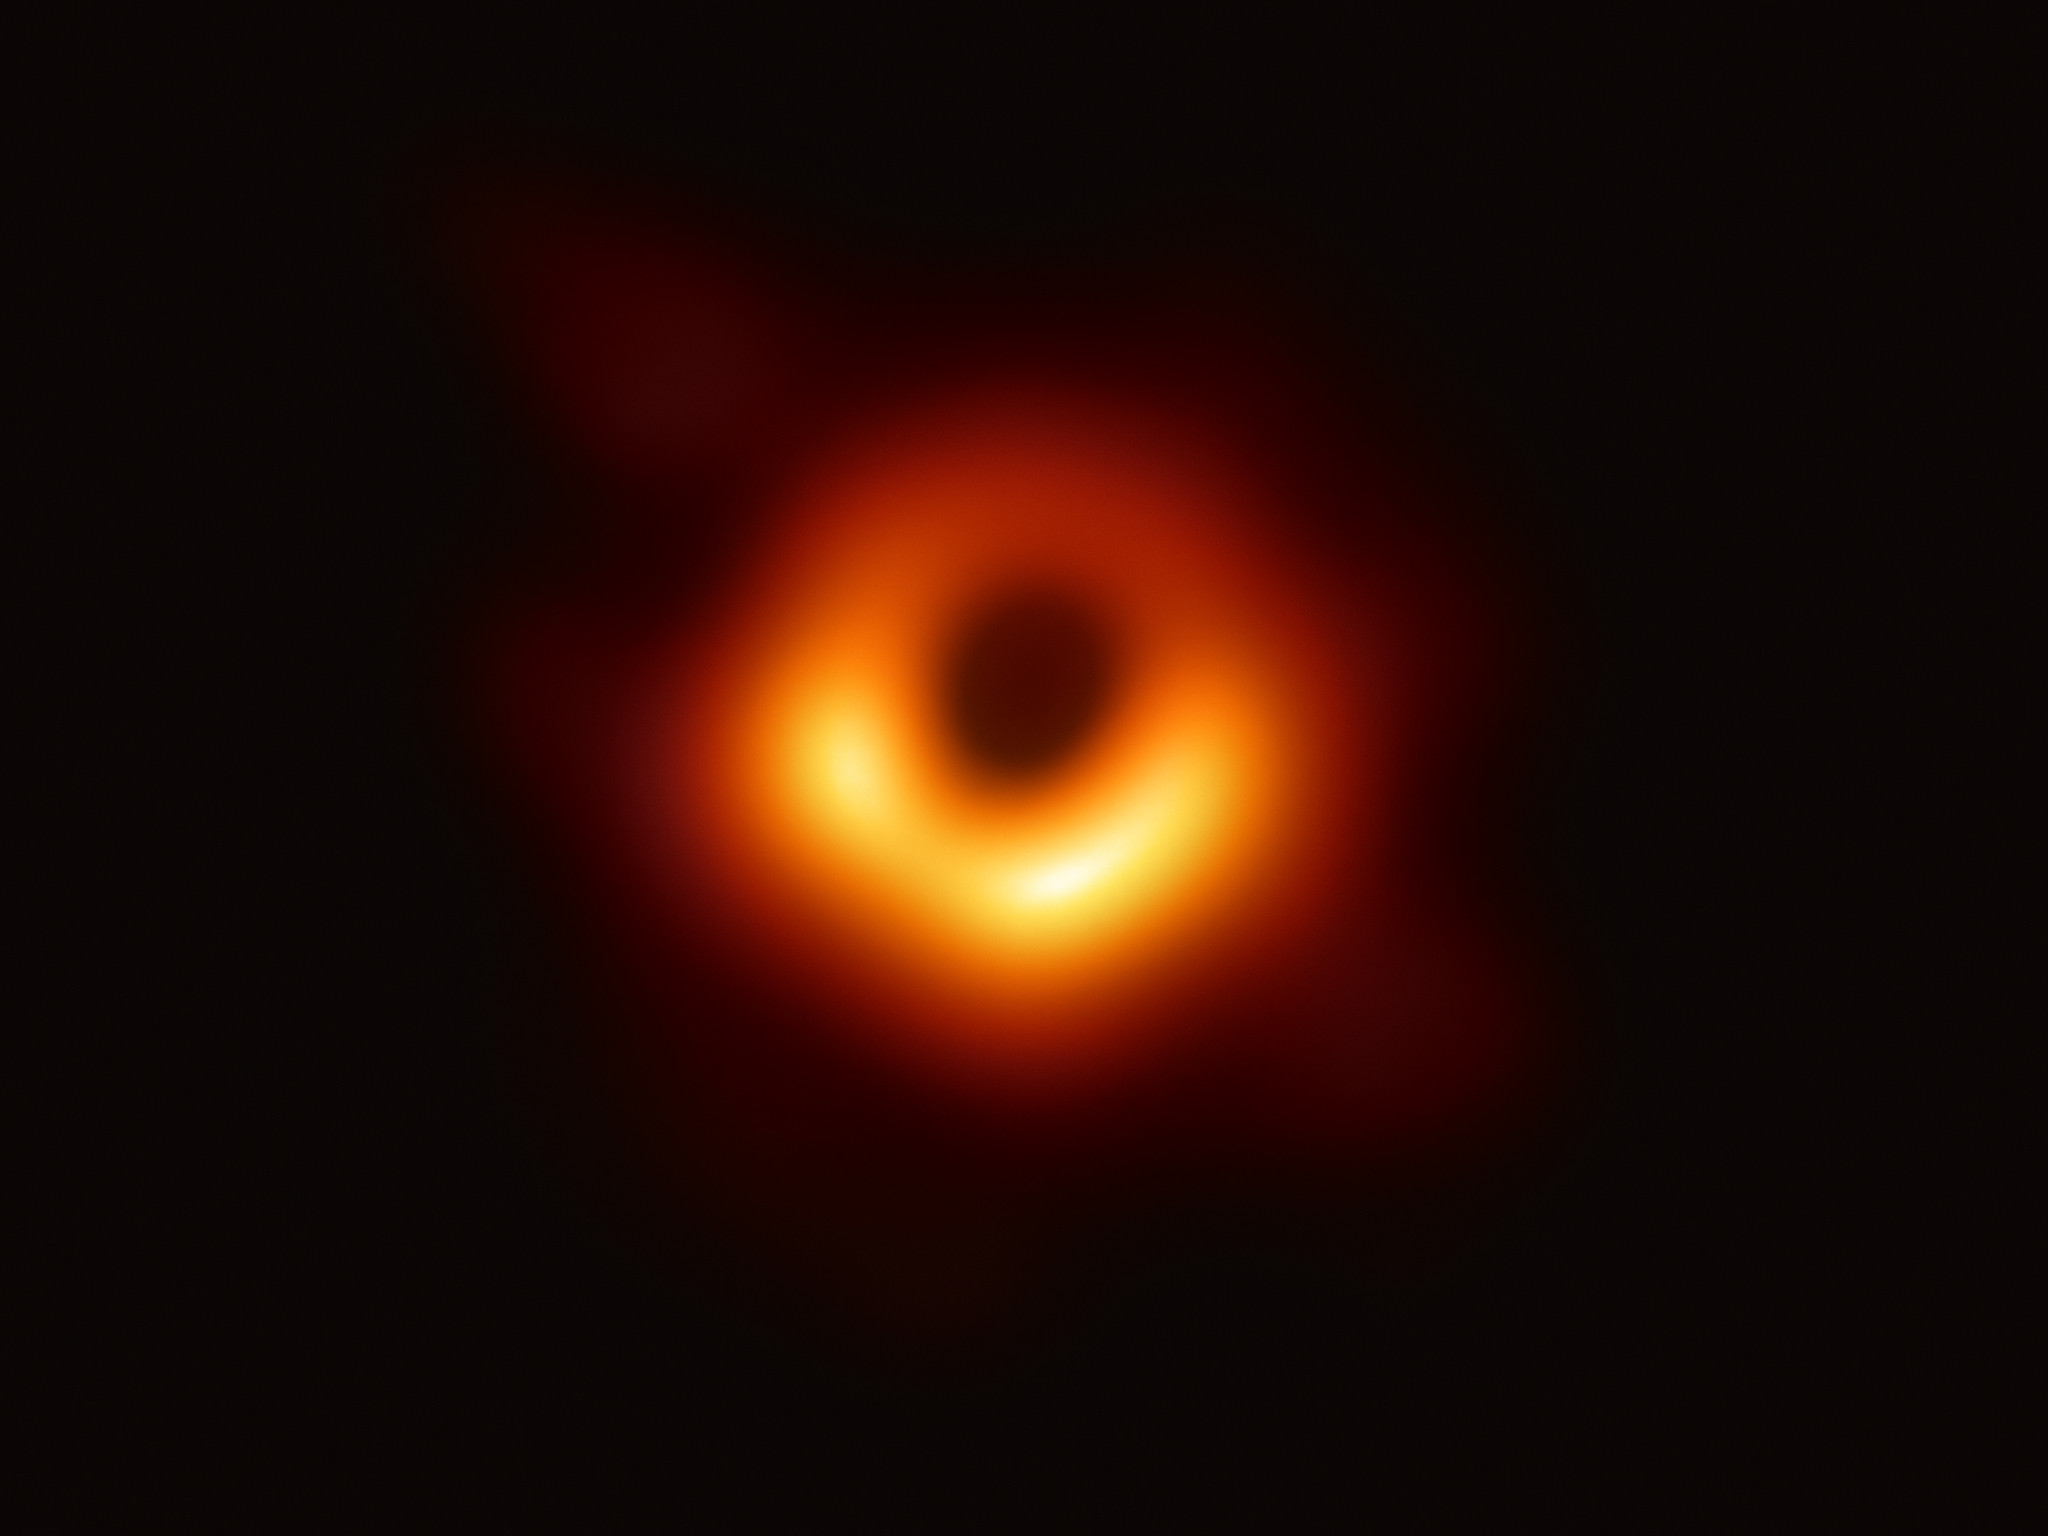
\includegraphics[width=0.7\textwidth]{pictures/blackhole.jpg}
    \caption{to jest zdjęcie prawdziwej czarnej dziury!}
    \label{fig:blackhole}
\end{figure}

\begin{table}[htbp]
\centering
\begin{tabular}{||c c c c||} 
 \hline
 Col1 & Col2 & Col3 & Col4 \\ [0.5ex] 
 \hline\hline
 774 & 885 & 996 & 117  \\
 \hline
 7   & 8   & 9   & 1  \\
 \hline
 7   & 8   & 9   & 1  \\
 \hline
 4   & 5   & 6   & 7  \\
 \hline
\end{tabular}
\label{tab:random_numbers}
\caption{TAB3LKA}
\end{table}

Wzory skróconego mnożenia:
\[(a+b)^2=a^2+2ab+b^2\]
\[(a-b)^2=a^2-2ab+b^2\]
I jeszcze takie:
$ a^2-b^2=(a-b)(a+b) $